\documentclass[10pt,a4paper]{article}
\usepackage[margin=1.7cm]{geometry}
\usepackage[T1]{fontenc}
\usepackage{lmodern}
\usepackage{xcolor}
\usepackage{booktabs}
\usepackage{array}
\usepackage{colortbl}
\usepackage{amsmath}
\usepackage{amssymb}
\usepackage{enumitem}
\usepackage{tabularx}
\usepackage{mdframed}
\usepackage{tikz}
\usetikzlibrary{positioning,arrows.meta,fit,backgrounds,shapes.geometric,calc}
\usepackage[colorlinks=true]{hyperref}

% ── Palette (shared with the rest of docs/) ───────────────────────────────────
\definecolor{hdrblue}{RGB}{10,60,140}
\definecolor{accentteal}{RGB}{0,120,120}
\definecolor{okgreen}{RGB}{20,110,40}
\definecolor{badred}{RGB}{180,20,20}
\definecolor{warnamber}{RGB}{180,90,0}
\definecolor{newbg}{RGB}{210,235,255}
\definecolor{newtext}{RGB}{0,60,130}
\definecolor{rulegray}{RGB}{130,130,130}
\definecolor{tablegray}{RGB}{245,246,248}
\definecolor{hwfill}{RGB}{222,236,255}
\definecolor{swfill}{RGB}{255,238,214}
\definecolor{goldfill}{RGB}{255,247,210}
\definecolor{deadfill}{RGB}{238,238,238}
\definecolor{warnbg}{RGB}{255,243,224}
\definecolor{okbg}{RGB}{223,244,228}

\hypersetup{linkcolor=hdrblue, urlcolor=accentteal,
  pdftitle={FPGA Tick-to-Trade: Is the Hardware in the Trades?}}

\setlength{\parindent}{0pt}
\setlength{\parskip}{4pt}

\newcommand{\sectionrule}{\par\nobreak\vspace{1pt}\textcolor{rulegray}{\rule{\linewidth}{0.8pt}}\par\vspace{1pt}}
\newcommand{\fpath}[1]{\texttt{\textcolor{hdrblue}{#1}}}

\newmdenv[linecolor=newtext, backgroundcolor=newbg, linewidth=1.2pt,
  leftmargin=0pt, rightmargin=0pt, innerleftmargin=8pt, innerrightmargin=8pt,
  innertopmargin=6pt, innerbottommargin=6pt, skipabove=6pt, skipbelow=6pt]{keybox}
\newmdenv[linecolor=badred, backgroundcolor=warnbg, linewidth=1.2pt,
  leftmargin=0pt, rightmargin=0pt, innerleftmargin=8pt, innerrightmargin=8pt,
  innertopmargin=6pt, innerbottommargin=6pt, skipabove=6pt, skipbelow=6pt]{warnboxx}
\newmdenv[linecolor=okgreen, backgroundcolor=okbg, linewidth=1.2pt,
  leftmargin=0pt, rightmargin=0pt, innerleftmargin=8pt, innerrightmargin=8pt,
  innertopmargin=6pt, innerbottommargin=6pt, skipabove=6pt, skipbelow=6pt]{okboxx}

\tikzset{
  hw/.style   ={rectangle, rounded corners=2pt, draw=hdrblue, fill=hwfill,
                text width=2.6cm, align=center, font=\footnotesize, minimum height=0.9cm, thick},
  sw/.style   ={rectangle, rounded corners=2pt, draw=warnamber, fill=swfill,
                text width=2.6cm, align=center, font=\footnotesize, minimum height=0.9cm, thick},
  dead/.style ={rectangle, rounded corners=2pt, draw=rulegray, fill=deadfill,
                text width=2.6cm, align=center, font=\footnotesize, minimum height=0.9cm, dashed, text=rulegray},
  src/.style  ={rectangle, rounded corners=2pt, draw=rulegray, fill=tablegray,
                text width=2.4cm, align=center, font=\footnotesize, minimum height=0.9cm},
  flow/.style ={-{Stealth[length=2.2mm]}, thick, draw=warnamber},
  noflow/.style={-{Stealth[length=2.2mm]}, thick, draw=rulegray, dashed},
}

\begin{document}

{\LARGE\bfseries\color{hdrblue} Is the Hardware in the Trades?}%
\hfill{\small\color{rulegray} 17 June 2026}\\[-2pt]
{\large\color{accentteal} What actually executes a live trade \textendash{} and what the RTL and Vivado work really bought}

\textcolor{hdrblue}{\rule{\linewidth}{2pt}}

% ── SHORT ANSWER ────────────────────────────────────────────────────────────────
\begin{warnboxx}
{\large\bfseries\color{badred} Short answer (the honest truth)}

\smallskip
The live paper trades you have run \textbf{do NOT use the FPGA hardware}. Every
trade was computed by the \textbf{Python software model}
(\fpath{host/strategy\_sw.py} + \fpath{host/risk\_guard.py}), running on your
CPU. \textbf{No \texttt{.sv} file executes during a trade, no bitstream exists,
and no FPGA (local or AWS F1) is in the loop.} The ``205\,ns'' printed next to
each signal is a \emph{hard-coded constant} (\fpath{FPGA\_LATENCY\_NS = 205})
copied from a \emph{simulation} result --- it is shown for comparison, not
measured live.

\smallskip
\textbf{So why does the project still mean something?} Because the software model
is \emph{provably identical} to the hardware (bit-for-bit, verified), and the
Vivado work \emph{proves the hardware is real and meets 200\,MHz timing}. The
trades are therefore exactly the decisions the FPGA \emph{would} make --- proven
by equivalence, not produced by silicon. The remaining step to put real silicon
in the loop is the AWS F1 build (Phase 3), which has not yet been done.
\end{warnboxx}

% ── 1. What actually runs ────────────────────────────────────────────────────────
{\large\bfseries\color{hdrblue} 1.\quad What Actually Runs During a Live Trade}
\sectionrule

When you run \fpath{python host/live\_feed.py -{}-alpaca -{}-execute}, the import
list tells the whole story --- it pulls in \emph{three Python modules and
nothing else}: \fpath{strategy\_sw}, \fpath{risk\_guard}, \fpath{ibkr\_bridge}.
There is no FPGA device handle, no PCIe/XDMA driver, no \texttt{.bit} or
\texttt{.awsxclbin} file loaded. The data path is 100\% software on the CPU:

\vspace{4pt}
\begin{center}
\resizebox{\linewidth}{!}{%
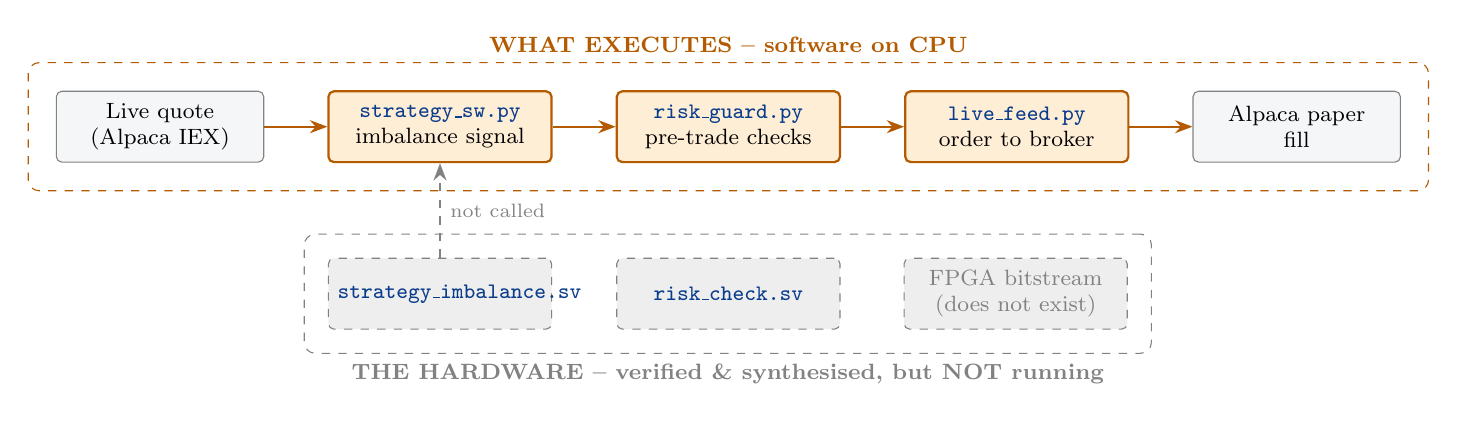
\begin{tikzpicture}[node distance=6mm and 8mm]
\node[src] (q) {Live quote\\ (Alpaca IEX)};
\node[sw, right=of q] (s) {\fpath{strategy\_sw.py}\\ imbalance signal};
\node[sw, right=of s] (r) {\fpath{risk\_guard.py}\\ pre-trade checks};
\node[sw, right=of r] (b) {\fpath{live\_feed.py}\\ order to broker};
\node[src, right=of b] (p) {Alpaca paper\\ fill};
\foreach \x/\y in {q/s,s/r,r/b,b/p} \draw[flow] (\x) -- (\y);

% the hardware, sitting OFF to the side, not connected
\node[dead, below=12mm of s] (hs) {\fpath{strategy\_imbalance.sv}};
\node[dead, below=12mm of r] (hr) {\fpath{risk\_check.sv}};
\node[dead, right=of hr] (hl) {FPGA bitstream\\ (does not exist)};
\draw[noflow] (hs) -- node[midway,right,font=\scriptsize,text=rulegray]{not called} (s);

\begin{scope}[on background layer]
  \node[fit=(q)(s)(r)(b)(p), draw=warnamber, dashed, rounded corners, inner sep=3.5mm,
        label={[warnamber,font=\footnotesize\bfseries]above:WHAT EXECUTES \textendash{} software on CPU}] {};
  \node[fit=(hs)(hr)(hl), draw=rulegray, dashed, rounded corners, inner sep=3mm,
        label={[rulegray,font=\footnotesize\bfseries]below:THE HARDWARE \textendash{} verified \& synthesised, but NOT running}] {};
\end{scope}
\end{tikzpicture}}
\end{center}

\begin{center}\small
\renewcommand{\arraystretch}{1.25}
\begin{tabularx}{\linewidth}{@{}>{\raggedright\arraybackslash}p{4.6cm} l X@{}}
\toprule
\textbf{Component} & \textbf{In a live trade?} & \textbf{Evidence} \\
\midrule
\fpath{strategy\_sw.py} (Python)      & \textcolor{okgreen}{\textbf{YES}} & imported \& called per quote \\
\fpath{risk\_guard.py} (Python)       & \textcolor{okgreen}{\textbf{YES}} & checks every order \\
\fpath{strategy\_imbalance.sv} (RTL)  & \textcolor{badred}{\textbf{NO}}   & never imported; RTL only runs in QuestaSim \\
\fpath{risk\_check.sv} (RTL)          & \textcolor{badred}{\textbf{NO}}   & same \\
Vivado-implemented design / bitstream & \textcolor{badred}{\textbf{NO}}   & no bitstream built; no FPGA present \\
The ``205\,ns'' figure                & \textcolor{warnamber}{\textbf{shown, not run}} & constant \fpath{FPGA\_LATENCY\_NS=205} from simulation \\
\bottomrule
\end{tabularx}
\end{center}

% ── 2. The three artifacts ───────────────────────────────────────────────────────
{\large\bfseries\color{hdrblue} 2.\quad Three Separate Artifacts \textendash{} and What Each One Is}
\sectionrule

The project produces \emph{three} representations of the same trading logic. They
are developed together but they \textbf{run in completely different places}.
Confusing them is the heart of your question, so here they are side by side:

\begin{center}\small
\renewcommand{\arraystretch}{1.3}
\begin{tabularx}{\linewidth}{@{}>{\raggedright\arraybackslash}p{3.0cm} X X@{}}
\toprule
\textbf{Artifact} & \textbf{Where it runs} & \textbf{What it proves / does} \\
\midrule
\textbf{(A) Python model}\newline \fpath{strategy\_sw.py}, \fpath{risk\_guard.py}
  & On your CPU, in \fpath{live\_feed.py}, on live market data.
  & Produces the \emph{actual} trades. This is the only thing that has touched a real (paper) market. \\
\textbf{(B) RTL in simulation}\newline \fpath{*.sv} in QuestaSim
  & Inside the QuestaSim simulator on your PC, driven by cocotb testbenches.
  & Proves the hardware \emph{logic} is correct (matches the golden model) and reports the \textbf{205\,ns} latency via \fpath{latency\_counter.sv}. This is a \emph{simulated} clock, not silicon. \\
\textbf{(C) RTL implemented in Vivado}\newline synthesised + placed \& routed netlist
  & Inside Vivado as a timing/area/power analysis. \emph{Not} downloaded to any chip.
  & Proves the same \texttt{.sv} is physically \emph{realisable}: it fits the VU9P, draws known power, and \textbf{closes timing at 200\,MHz}. This is what makes the 205\,ns \emph{credible} rather than a guess. \\
\bottomrule
\end{tabularx}
\end{center}

\begin{keybox}
The trades are artifact \textbf{(A)}. The ``hardware'' is artifacts \textbf{(B)}
and \textbf{(C)} --- both verified, neither \emph{executing} a trade. There is no
fourth artifact (a running FPGA) yet; that is the AWS F1 step still to do.
\end{keybox}

% ── 3. How the hardware is "included": equivalence, not execution ─────────────────
{\large\bfseries\color{hdrblue} 3.\quad How the Hardware Is ``Included'' \textendash{} by Equivalence}
\sectionrule

The hardware is connected to the trades by a \textbf{proven equivalence chain},
not by execution. Each link is verified so that ``what the software decided'' and
``what the FPGA would have decided'' are guaranteed identical:

\vspace{4pt}
\begin{center}
\resizebox{\linewidth}{!}{%
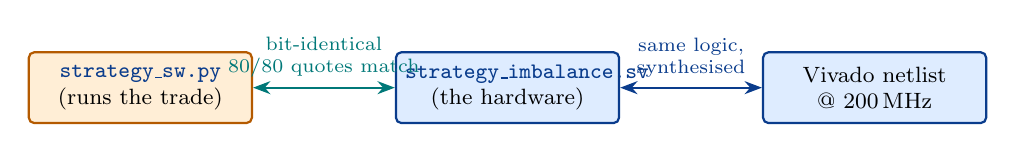
\begin{tikzpicture}[node distance=10mm]
\node[sw] (a) {\fpath{strategy\_sw.py}\\ (runs the trade)};
\node[hw, right=18mm of a] (b) {\fpath{strategy\_imbalance.sv}\\ (the hardware)};
\node[hw, right=18mm of b] (c) {Vivado netlist\\ @ 200\,MHz};
\draw[{Stealth[length=2.2mm]}-{Stealth[length=2.2mm]}, thick, draw=accentteal]
   (a) -- node[midway,above,font=\scriptsize,align=center,text=accentteal]{bit-identical\\ 80/80 quotes match} (b);
\draw[{Stealth[length=2.2mm]}-{Stealth[length=2.2mm]}, thick, draw=hdrblue]
   (b) -- node[midway,above,font=\scriptsize,align=center,text=hdrblue]{same logic,\\ synthesised} (c);
\end{tikzpicture}}
\end{center}

\begin{itemize}[leftmargin=1.4em, topsep=2pt, itemsep=1pt]
\item \textbf{Software $\equiv$ RTL.} \fpath{tb\_shadow\_quotes.py} feeds the
  \emph{same} quote stream to \fpath{strategy\_sw.py} and to the RTL in QuestaSim
  and diffs every decision: \textbf{80/80 quotes matched, 44 software signals =
  44 RTL signals, 0 mismatches} (\fpath{reports/shadow\_report.csv}). The Python
  model is therefore a faithful stand-in for the gate-level behaviour.
\item \textbf{RTL $\equiv$ implemented design.} Vivado synthesis + place-and-route
  turn that exact \texttt{.sv} into a gate-level netlist and confirm it behaves
  identically (functional gate sim, \fpath{gatesim/}) while meeting timing.
\end{itemize}

So when a trade fires, you can correctly say: \emph{``this is the decision the
FPGA would produce in 205\,ns,''} because (A) $\equiv$ (B) $\equiv$ (C) is proven.
What you cannot yet say is \emph{``the FPGA produced this decision''} --- because
no FPGA ran it.

% ── 4. What Vivado synthesis & implementation actually bought ─────────────────────
{\large\bfseries\color{hdrblue} 4.\quad What the Vivado Synthesis \& Implementation Bought}
\sectionrule

It is fair to ask: if the bitstream never ran, what was the point of the Vivado
work? It is what separates a \emph{real hardware design} from a Python script that
merely \emph{claims} it would be fast. Vivado provided hard, measured evidence:

\begin{center}\small
\renewcommand{\arraystretch}{1.25}
\begin{tabularx}{\linewidth}{@{}>{\raggedright\arraybackslash}p{4.2cm} X@{}}
\toprule
\textbf{Vivado output} & \textbf{What it establishes} \\
\midrule
\textbf{Timing closure} (WNS \textbf{+0.105\,ns}, 0 failing endpoints @ 200\,MHz)
  & The design genuinely runs at 200\,MHz $\Rightarrow$ the 5\,ns clock period is real $\Rightarrow$ 41 cycles \emph{is} 205\,ns. Without this, ``205\,ns'' would be an unproven assumption. \\
\textbf{Resource usage} (\textasciitilde7{,}043 LUTs, 4{,}576 FFs, 1 BRAM, 0 DSP for \fpath{tick\_to\_trade\_top})
  & The logic fits the VU9P with vast headroom $\Rightarrow$ it is buildable, and scalable to multi-symbol (\textasciitilde20\,k LUTs for 4 symbols). \\
\textbf{Power} (\textasciitilde2.6\,W total)
  & Realistic, deployable power envelope. \\
\textbf{Gate-level netlist} (\fpath{gatesim/})
  & Post-synthesis functional sim confirms the synthesised gates behave like the source RTL --- the logic survives the translation to hardware primitives. \\
\bottomrule
\end{tabularx}
\end{center}

\begin{keybox}
In short: \textbf{simulation (B) proves the logic is correct and measures 205\,ns;
Vivado (C) proves that 205\,ns is physically achievable on the real device.}
Together they make the latency claim trustworthy. They do not, by themselves, put
the chip in the trading loop.
\end{keybox}

% ── 5. The three latency numbers ─────────────────────────────────────────────────
{\large\bfseries\color{hdrblue} 5.\quad The Three Latency Numbers \textendash{} Don't Mix Them Up}
\sectionrule

\begin{center}\small
\renewcommand{\arraystretch}{1.3}
\begin{tabularx}{\linewidth}{@{}l l X@{}}
\toprule
\textbf{Number} & \textbf{Source} & \textbf{Meaning} \\
\midrule
\textbf{205\,ns} & RTL in QuestaSim (\fpath{tb\_phase3\_pipeline.py}) + Vivado timing
  & Simulated tick-to-trade of the hardware, validated as physically achievable. \emph{Not} measured on silicon. \\
\textbf{\textasciitilde9\,$\mu$s} & Live run, \fpath{time.perf\_counter\_ns} around \fpath{strategy\_sw.evaluate}
  & The \emph{actual} software compute latency on your CPU during real trades --- the only one measured live. \\
\textbf{\textasciitilde$\,$tens of ms} & Network round-trip to the broker
  & The dominant real-world delay on the live order path. \\
\bottomrule
\end{tabularx}
\end{center}

The headline ``$\sim$45$\times$ faster on hardware'' compares 205\,ns (B/C) to the
$\approx$9\,$\mu$s software compute (the live measurement) --- an
\emph{apples-to-apples compute} comparison of the same logic on two substrates.

% ── 6. What would put silicon in the loop ────────────────────────────────────────
{\large\bfseries\color{hdrblue} 6.\quad What Would Make the FPGA Actually Execute Trades}
\sectionrule

\begin{okboxx}
To move from ``the FPGA \emph{would} decide this'' to ``the FPGA \emph{did} decide
this,'' the remaining work (Phase 3, all gated on AWS) is:
\begin{enumerate}[leftmargin=1.5em, topsep=2pt, itemsep=1pt]
\item Build an \textbf{AFI} (Amazon FPGA Image) from \fpath{f1/cl\_tick\_to\_trade.sv}
      on an EC2 FPGA Developer instance (full Vivado Shell build).
\item Launch an \textbf{f1.2xlarge} and load the AFI onto the VU9P.
\item DMA/stream ITCH into the device and read decisions + the real latency
      histogram back via \fpath{f1/host\_replay.py -{}-device}.
\item Diff the silicon decisions against the golden model and confirm
      \textbf{$\approx$205\,ns on real hardware}.
\end{enumerate}
Only after step 4 is the 205\,ns a \emph{silicon-measured} number and the FPGA
genuinely in the decision path. The local clone has \textbf{no bitstream} today,
which is why none of the live trades touched hardware.
\end{okboxx}

\vfill
{\small\color{rulegray} Companion: \fpath{project\_complete\_flow.pdf} (full
flow), \fpath{implementation\_results.pdf} (Vivado timing/area/power),
\fpath{validation\_roadmap.pdf} (the 4 phases). Build:
\texttt{pdflatex hardware\_in\_the\_loop.tex}.}

\end{document}
